\section{Projections of differential Higgs boson production cross sections and interpretations thereof}

\tk{TODO}


\subsection{High-Luminosity LHC}

\tk{TODO}


\subsection{Scenarios for the systematic uncertainties at \texorpdfstring{$3000\fbinv$}{3000 fb-1}}

\tk{TODO}


\subsection{Projections for the  \texorpdfstring{$\pth$}{pT(H)} spectrum and its interpretations}

\tk{TODO: This is the literal PAS text}

The measurement of Higgs boson differential cross sections can provide constraints on physical parameters that have a small effect on inclusive quantities such as total cross sections, but cause larger deviations in the distributions of certain observables.
% 
By varying the Higgs couplings, the strength with which quarks and other bosons couple to the Higgs boson, significant distortions in the shapes of differential cross sections appear, in particular for the transverse momentum distribution.
% 
The combination of differential cross sections from the \hgg, \hzz and boosted gluon-fusion-induced \hbb, along with an interpretation in the $\kappa$-framework~\cite{LHCHXSWGYR3}, is documented in Ref.~\cite{CMS-PAS-HIG-17-028}.
% 
This section describes the projected results of the differential spectra and fits of the Higgs coupling modifiers.
% 
The projected differential cross section is only computed for $\pth$, for each of the individual decay channels and for the combination.
% 
The cross sections in all bins are determined from a simultaneous maximum likelihood fit as described in section~\ref{sec:stat}. The unfolding of the number of observed events in each bin to the particle level, to account for detector effects and bin-to-bin migrations, is performed within this fit.

% ____________________________________________________________________________
\subsubsection{The differential cross section for \texorpdfstring{$\pth$}{pTH}}

The projection of the differential cross section for the $\pth$ spectrum is shown in Fig.~\ref{fig:proj_pth}, for both S1 and S2.
% 
The relative uncertainties for both scenarios are given in Tables~\ref{tab:proj_pth_unc_scen1} and \ref{tab:proj_pth_unc_scen2}.
% 
With respect to the uncertainties at the current integrated luminosity of 35.9\fbinv, the uncertainties at 3000\fbinv in the higher $\pth$ region are about a factor of ten smaller. This is expected, as the uncertainties in this region remain statistically dominated.
% 
The uncertainties in the lower $\pth$ region are no longer statistically dominated however, as can been seen by comparing Table~\ref{tab:proj_pth_unc_scen1} with Table~\ref{tab:proj_pth_unc_scen2}, where the reduced systematic uncertainties in S2 yield a reduction in the total uncertainty of up to 25\% compared to S1.


\begin{figure}[hbtp]
  \begin{center}
    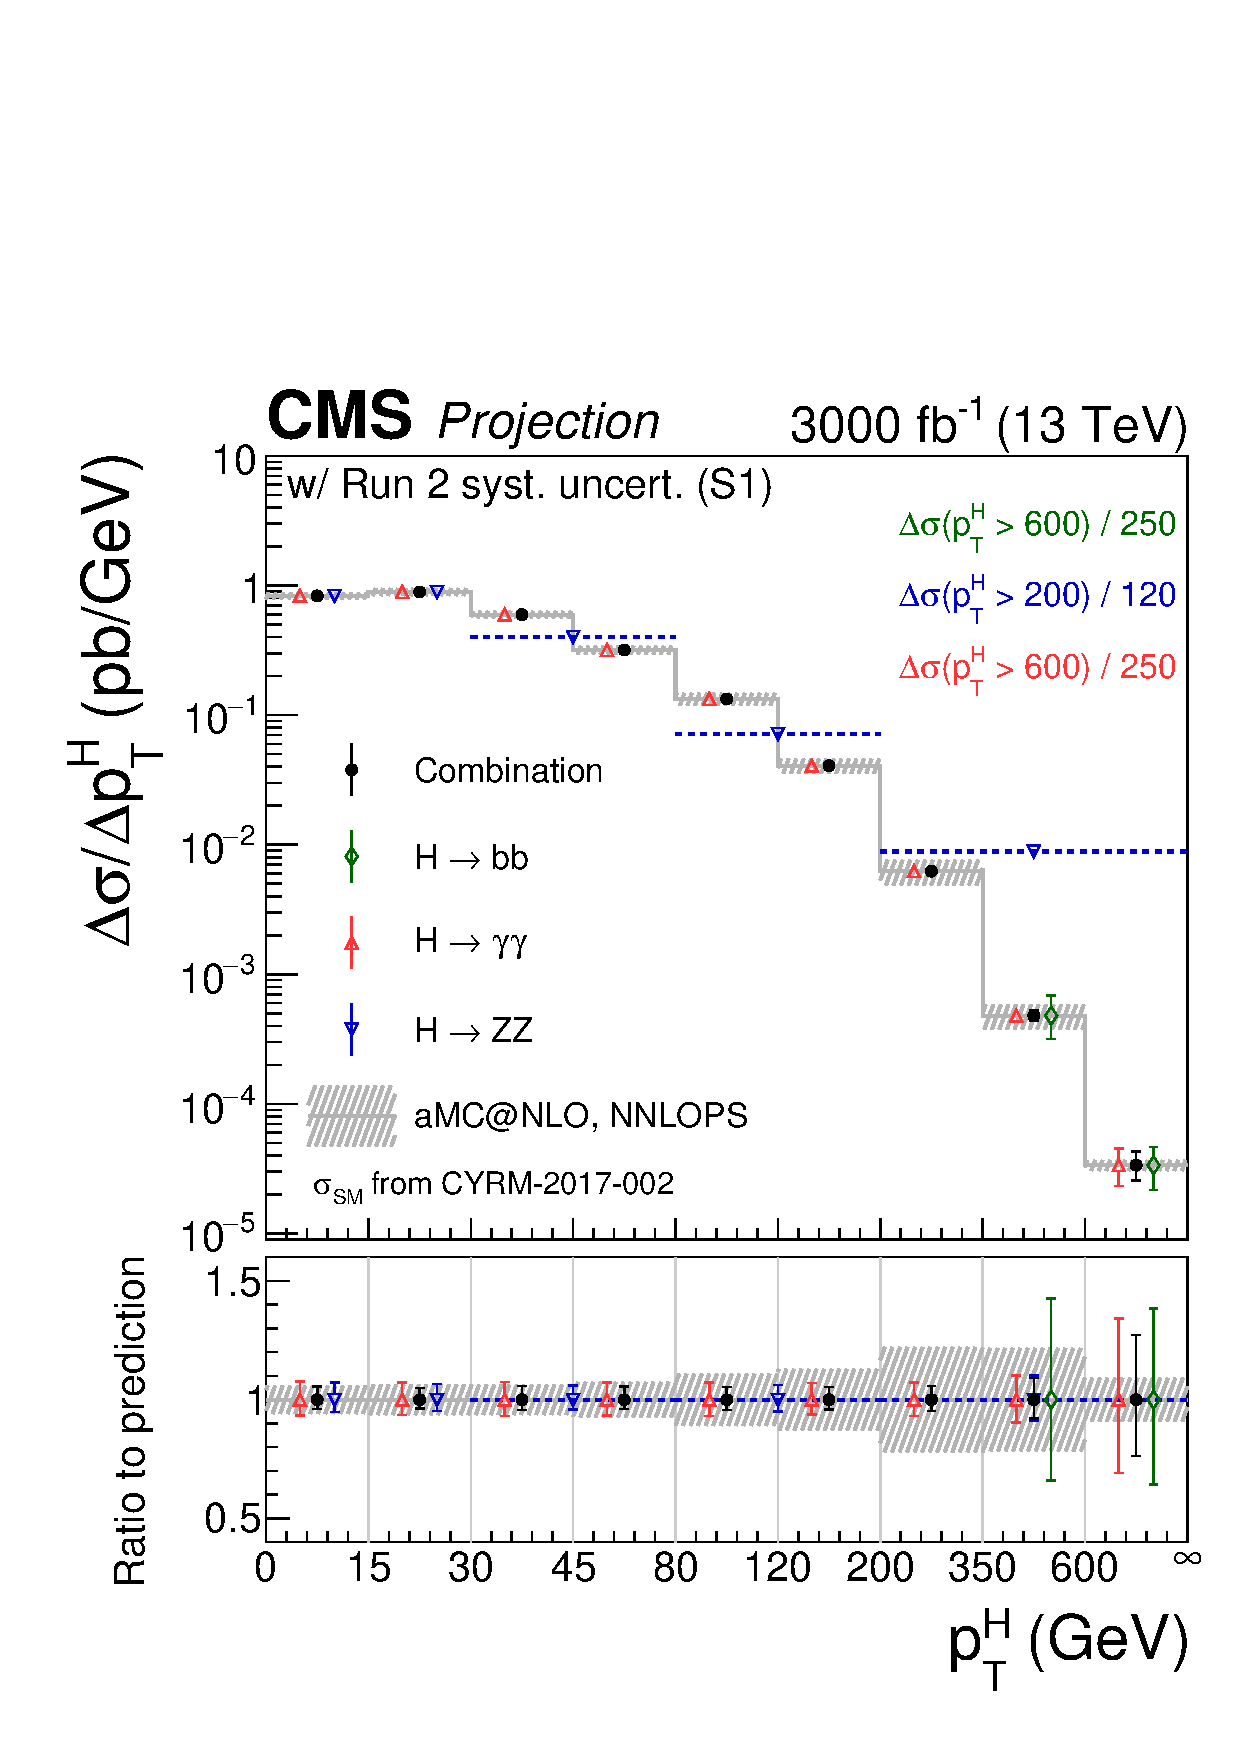
\includegraphics[width=0.49\linewidth]{img/projections/projectionspectra_pth_smH.pdf}
    % \includegraphics[width=0.49\linewidth]{img/projections/projectionspectra_pth_smH_statonly.pdf}
    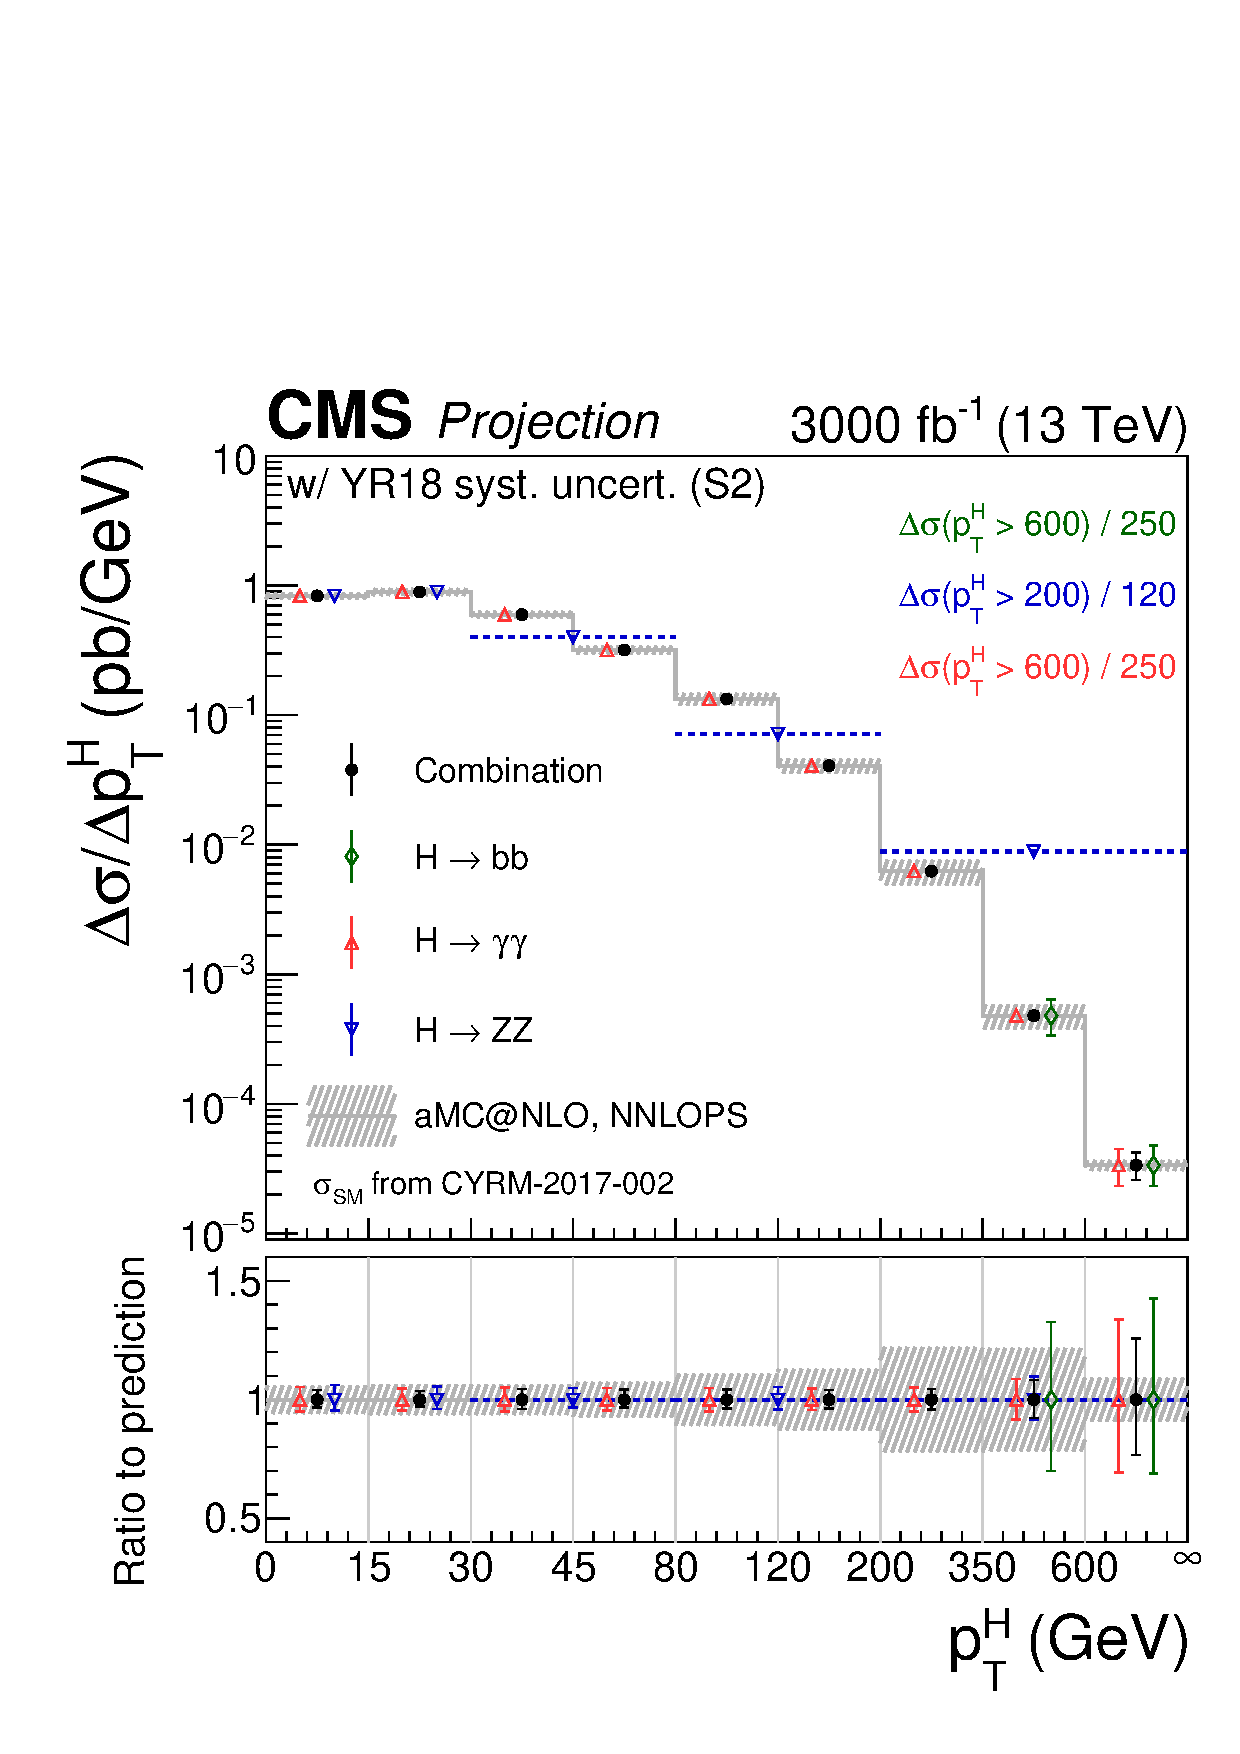
\includegraphics[width=0.49\linewidth]{img/projections/projectionspectra_pth_smH_scenario2.pdf}
    \caption{
        Projected differential cross section for the $\pth$ spectrum at an integrated luminosity of 3000\fbinv, under S1 (left, with Run~2 systematic uncertainties~\cite{CMS-PAS-HIG-17-028}) and S2 (right, with YR18 systematic uncertainties).
        }
    \label{fig:proj_pth}
  \end{center}
\end{figure}


\begin{table}[htb]
\footnotesize
\begin{center}
\begin{tabular}{|l|c|c|c|c|c|c|c|c|c|}
\hline
$\pth$       & 0-15    &  15-30   &  30-45    &  45-80   &  80-120  &  120-200  &  200-350  &  350-600  &  600-$\infty$  \\
\hline
$\hgg$       & 7.16\%  &  6.82\%  &  7.13\%   &  6.94\%  &  7.05\%  &  6.65\%   &  7.09\%   &  9.87\%   &  32.55\%  \\
\hline
$\hzz$       & 6.21\%  &  5.66\%  &  \multicolumn{2}{c|}{5.02\%}  &  \multicolumn{2}{c|}{5.55\%}  &  \multicolumn{3}{c|}{9.56\%} \\
\hline
$\hbb$       & \multicolumn{7}{c|}{\textit{None}}                                                       &  38.22\%  &  37.11\%  \\
\hline
Combination  & 4.70\%  &  4.36\%  &  5.04\%   &  4.66\%  &  4.84\%  &  4.73\%   &  5.23\%   &  8.53\%   &  25.45\%  \\
\hline
\end{tabular}
\end{center}
\caption{
    Relative uncertainties on the projected $\pth$ spectrum under S1 (with Run~2 systematic uncertainties~\cite{CMS-PAS-HIG-17-028}) at $3000\fbinv$.
    }
\label{tab:proj_pth_unc_scen1}
\end{table}

\begin{table}[htb]
\footnotesize
\begin{center}
\begin{tabular}{|l|c|c|c|c|c|c|c|c|c|}
\hline
$\pth$       & 0-15    &  15-30   &  30-45    &  45-80   &  80-120  &  120-200  &  200-350  &  350-600  &  600-$\infty$  \\
\hline
$\hgg$       &  5.12\%  &   4.55\%  &  5.10\%   &   4.78\%   &   4.94\%   &   4.52\%   &  5.10\%   &  8.57\%   &   32.24\%    \\
\hline
$\hzz$       &  5.36\%  &   4.80\%  &  \multicolumn{2}{c|}{4.06\%}   &   \multicolumn{2}{c|}{4.71\%}   &   \multicolumn{3}{c|}{9.10\%}  \\
\hline
$\hbb$       &  \multicolumn{7}{c|}{\textit{None}}                                                             &  31.41\%  &   36.81\%    \\
\hline
Combination  &  3.72\%  &   3.26\%  &  4.22\%   &   3.75\%   &   3.97\%   &   3.83\%   &  4.37\%   &  8.04\%   &   24.54\%    \\
\hline
\end{tabular}
\end{center}
\caption{
    Relative uncertainties on the projected $\pth$ spectrum under S2 (with YR18 systematic uncertainties) at $3000\fbinv$.
    }
\label{tab:proj_pth_unc_scen2}
\end{table}

% \begin{table}[htb]
% \footnotesize
% \begin{center}
% \begin{tabular}{|l|c|c|c|c|c|c|c|c|c|}
% \hline
% $\pth$       & 0-15    &  15-30   &  30-45    &  45-80   &  80-120  &  120-200  &  200-350  &  350-600  &  600-$\infty$  \\
% \hline
% $\hgg$       &  4.06\%  &  3.24\%  &  4.02\%  &  3.55\%  &  3.77\%  &  3.33\%   &  4.07\%  &  7.99\%   &  32.09\%    \\
% \hline
% $\hzz$       &  4.19\%  &  3.91\%  &  \multicolumn{2}{c|}{3.01\%}  &  \multicolumn{2}{c|}{3.88\%} &  \multicolumn{3}{c|}{8.79\%}  \\
% \hline
% $\hbb$       &  \multicolumn{7}{c|}{\textit{None}}                                                   &  25.63\%  &  30.59\%    \\
% \hline
% Combination  &  2.92\%  &  2.50\%  &  3.67\%  &  3.11\%  &  3.36\%  &  3.20\%   &  3.79\%  &  7.61\%   &  22.25\%    \\
% \hline
% \end{tabular}
% \end{center}
% \caption{
%     Relative uncertainties on the projected $\pth$ spectrum assuming vanishing systematic uncertainties.
%     }
% \label{tab:proj_pth_unc_scen3}
% \end{table}


% ____________________________________________________________________________
\subsubsection{Constraining Higgs coupling modifiers using the \texorpdfstring{$\pth$}{pTH} spectrum}

Theoretical predictions of differential distributions can be fitted to data, and can subsequently be used to constrain physical parameters such as couplings of the Higgs.
% 
Two sets of parametrizations are fitted to the projected $\pth$ distribution: 
% 
Parametrizations dependent on $\kappa_\textrm{b}$ and $\kappa_\textrm{c}$, computed in Ref.~\cite{Bishara:2016jga}, and parametrizations dependent on $\kappa_\textrm{t}$ and $c_\textrm{g}$, computed in Ref.~\cite{Grazzini:2017szg,Grazzini:2016paz}.
% 
The calculations of the former extend up to 120\GeV in $\pth$, and therefore $\hbb$ is not used in the fit.
% 
The results of the fits of $\kappa_\textrm{b}$/$\kappa_\textrm{c}$ and $\kappa_\textrm{t}$/$c_\textrm{g}$ are shown in Fig.~\ref{fig:proj_kbkc} and Fig.~\ref{fig:proj_ktcg} respectively.
% 
Additional theoretical uncertainties on the differential cross section predictions are included in the systematic uncertainties, and are not reduced with integrated luminosity.
% 
For this reason, the relative difference between S1 and S2 is expected not to be as pronounced as in the case of the differential $\pth$ combination.


\begin{figure}[hbtp]
  \begin{center}
    \ifbool{draftmode}{
        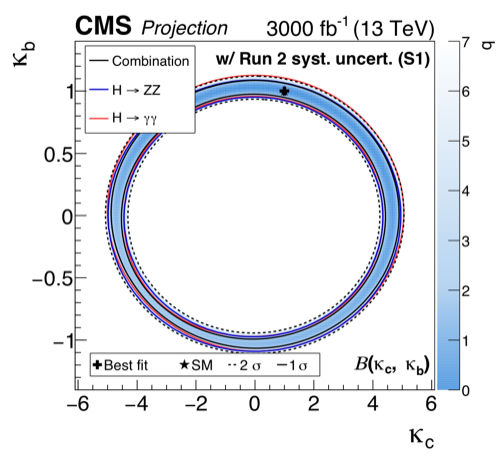
\includegraphics[width=0.49\linewidth]{img/projections/projection_kbkc_plot_couplingdependentBRs.png}
        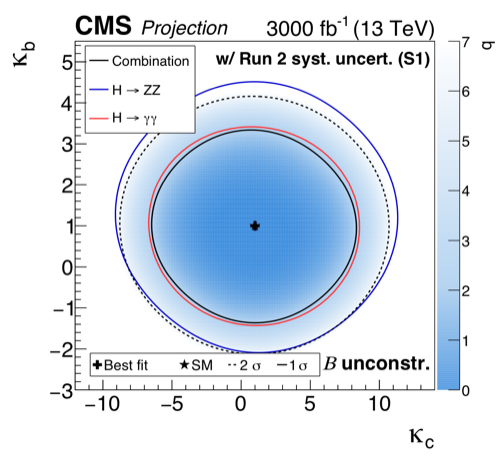
\includegraphics[width=0.49\linewidth]{img/projections/projection_kbkc_plot_floatingBRs.png}
        % 
        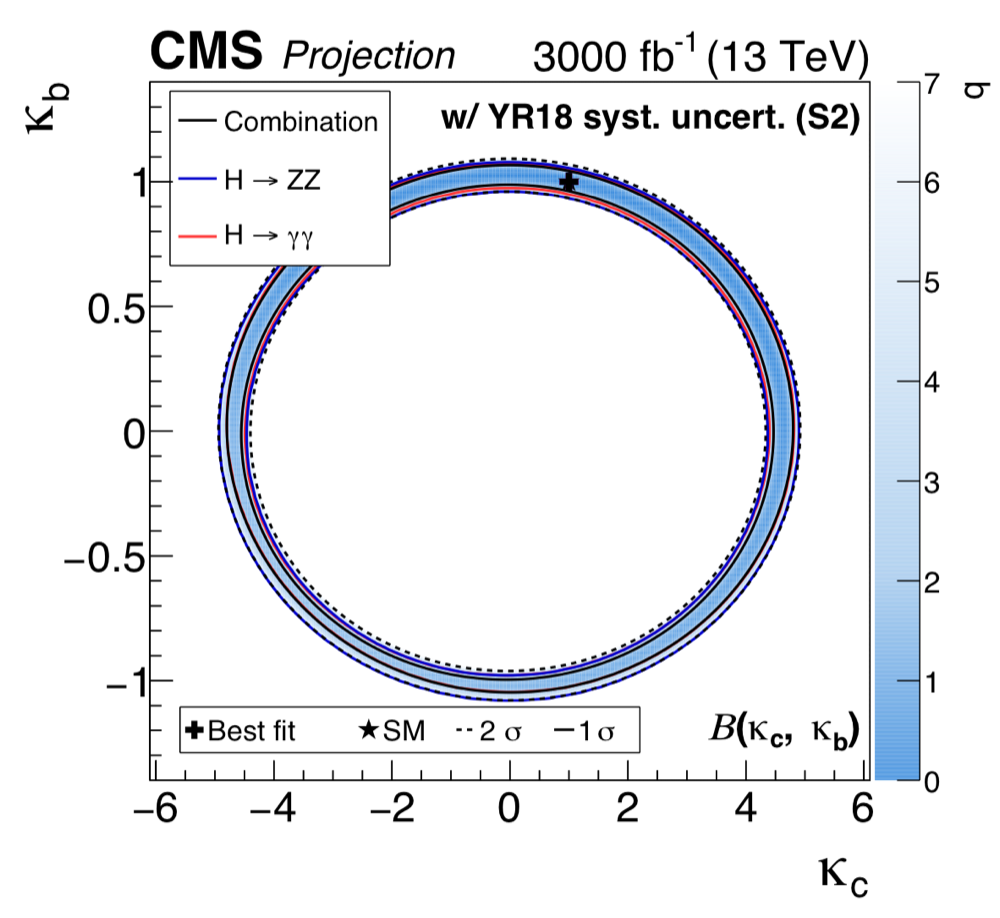
\includegraphics[width=0.49\linewidth]{img/projections/projection_kbkc_plot_couplingdependentBRs_scenario2.png}
        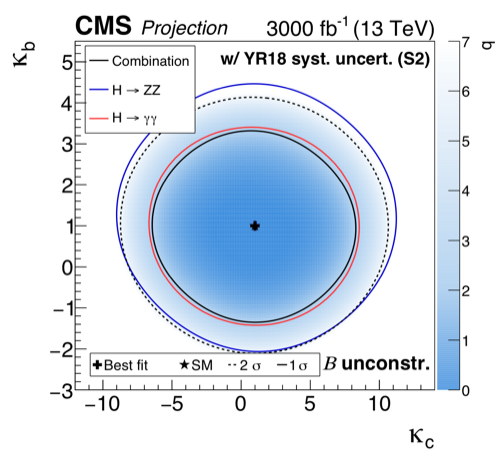
\includegraphics[width=0.49\linewidth]{img/projections/projection_kbkc_plot_floatingBRs_scenario2.png}
        }{
        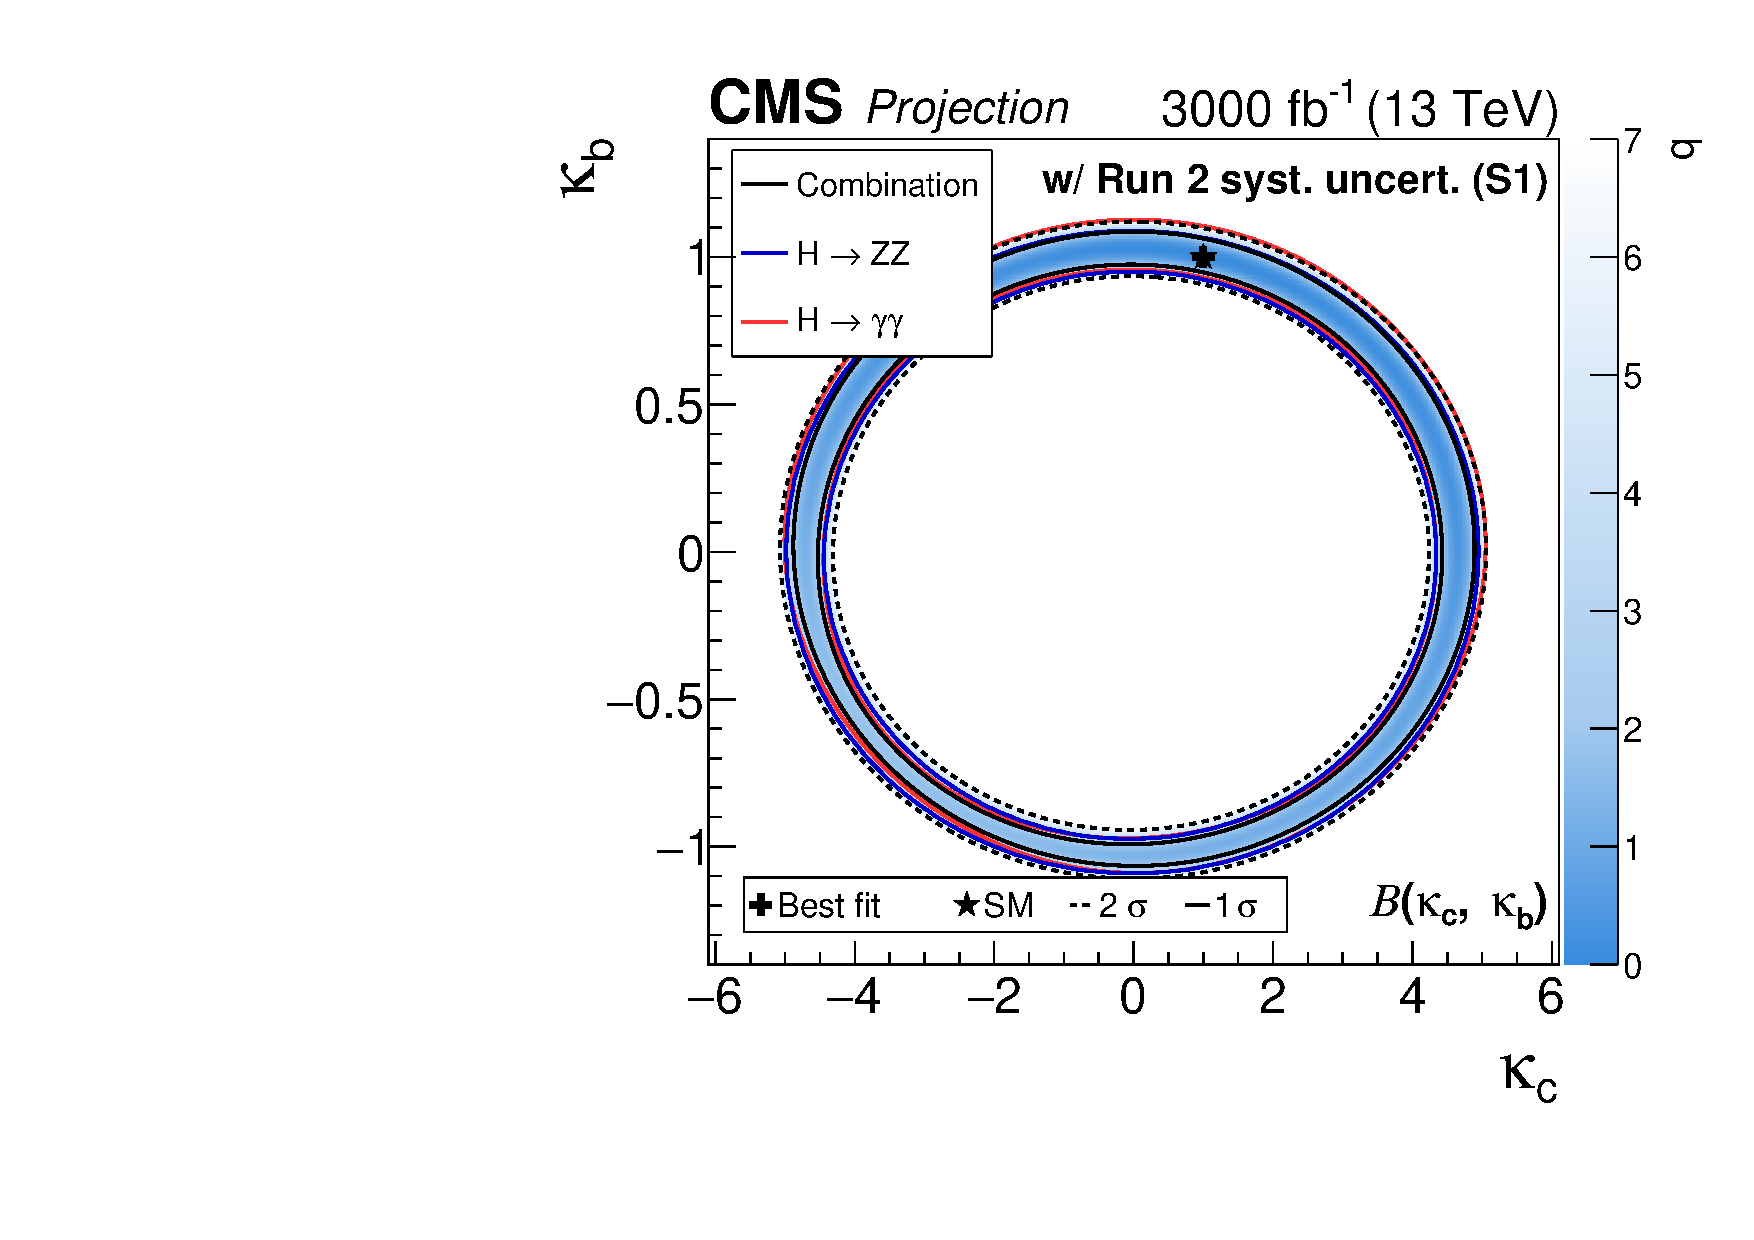
\includegraphics[width=0.49\linewidth]{img/projections/projection_kbkc_plot_couplingdependentBRs.pdf}
        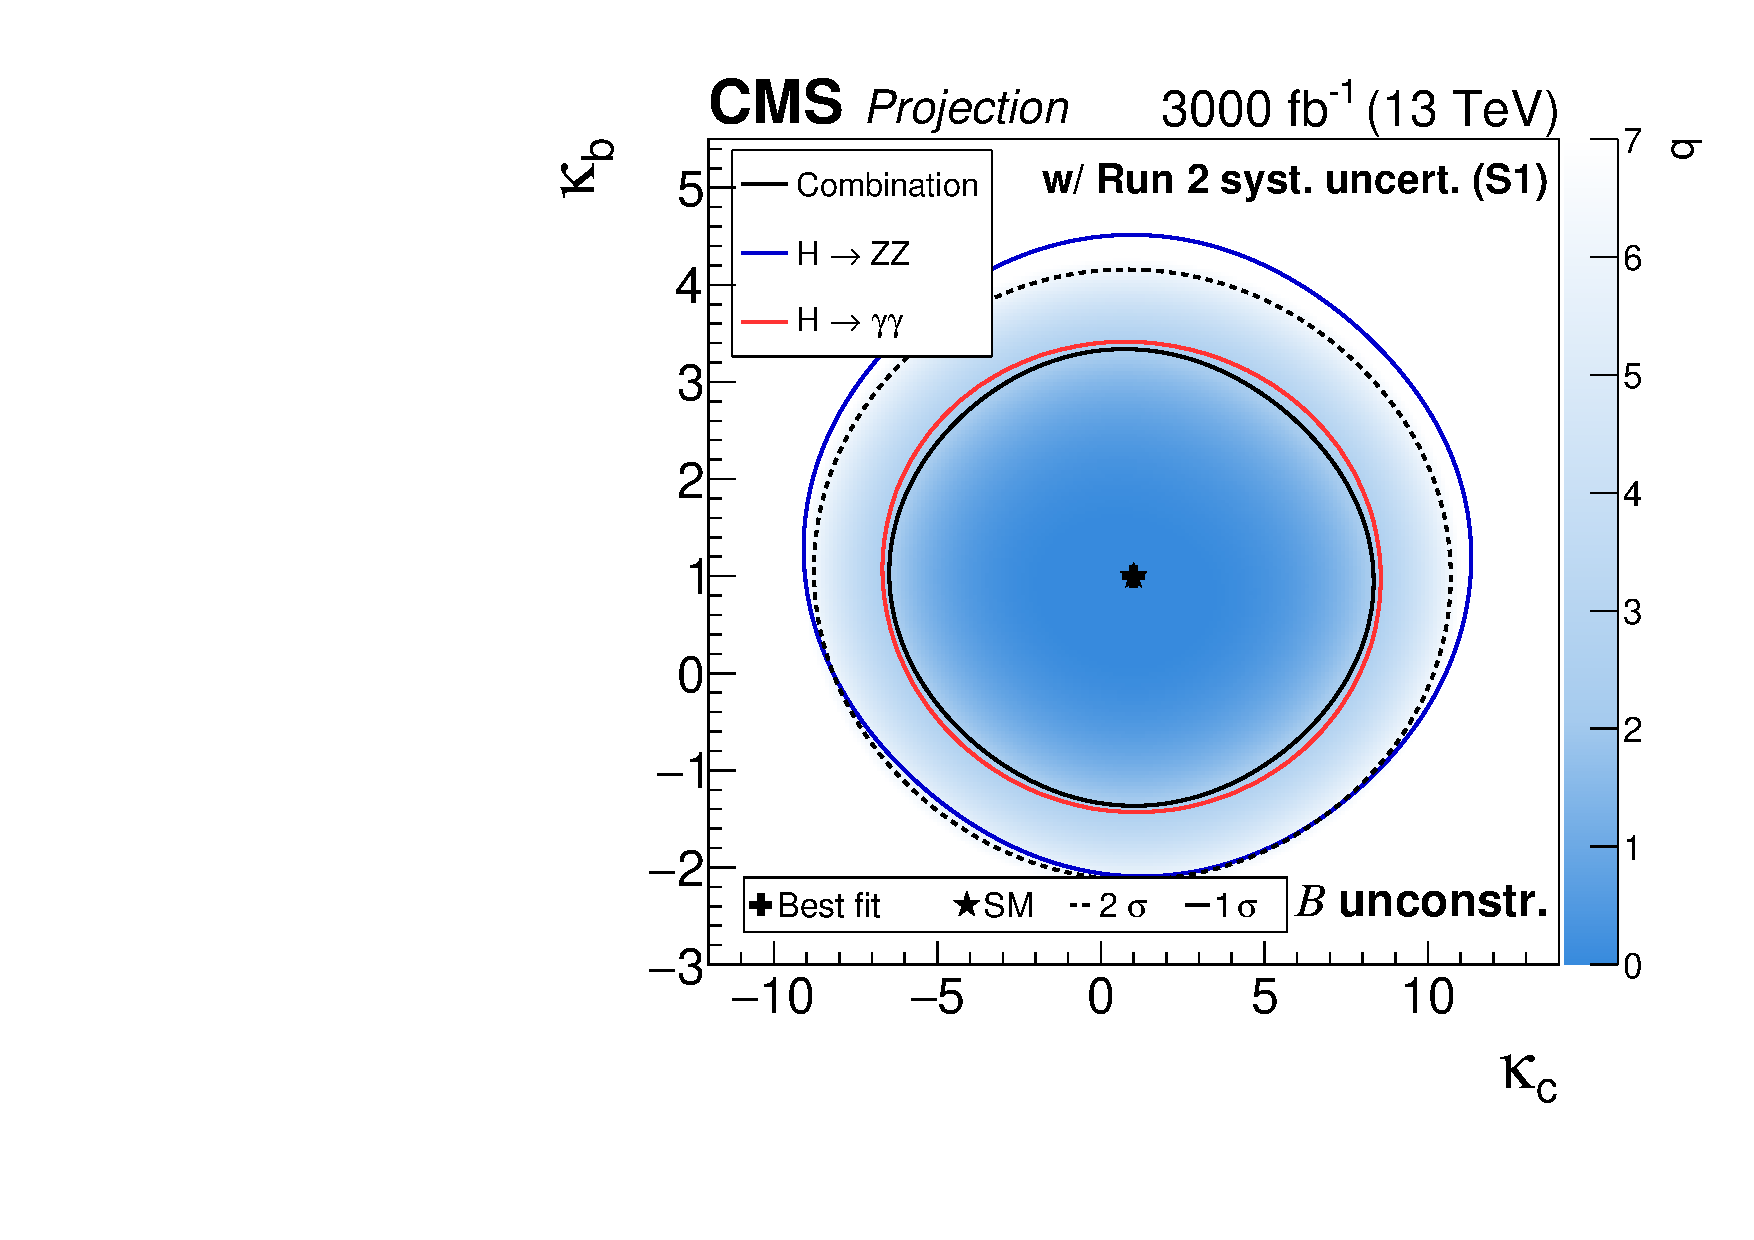
\includegraphics[width=0.49\linewidth]{img/projections/projection_kbkc_plot_floatingBRs.pdf}
        % 
        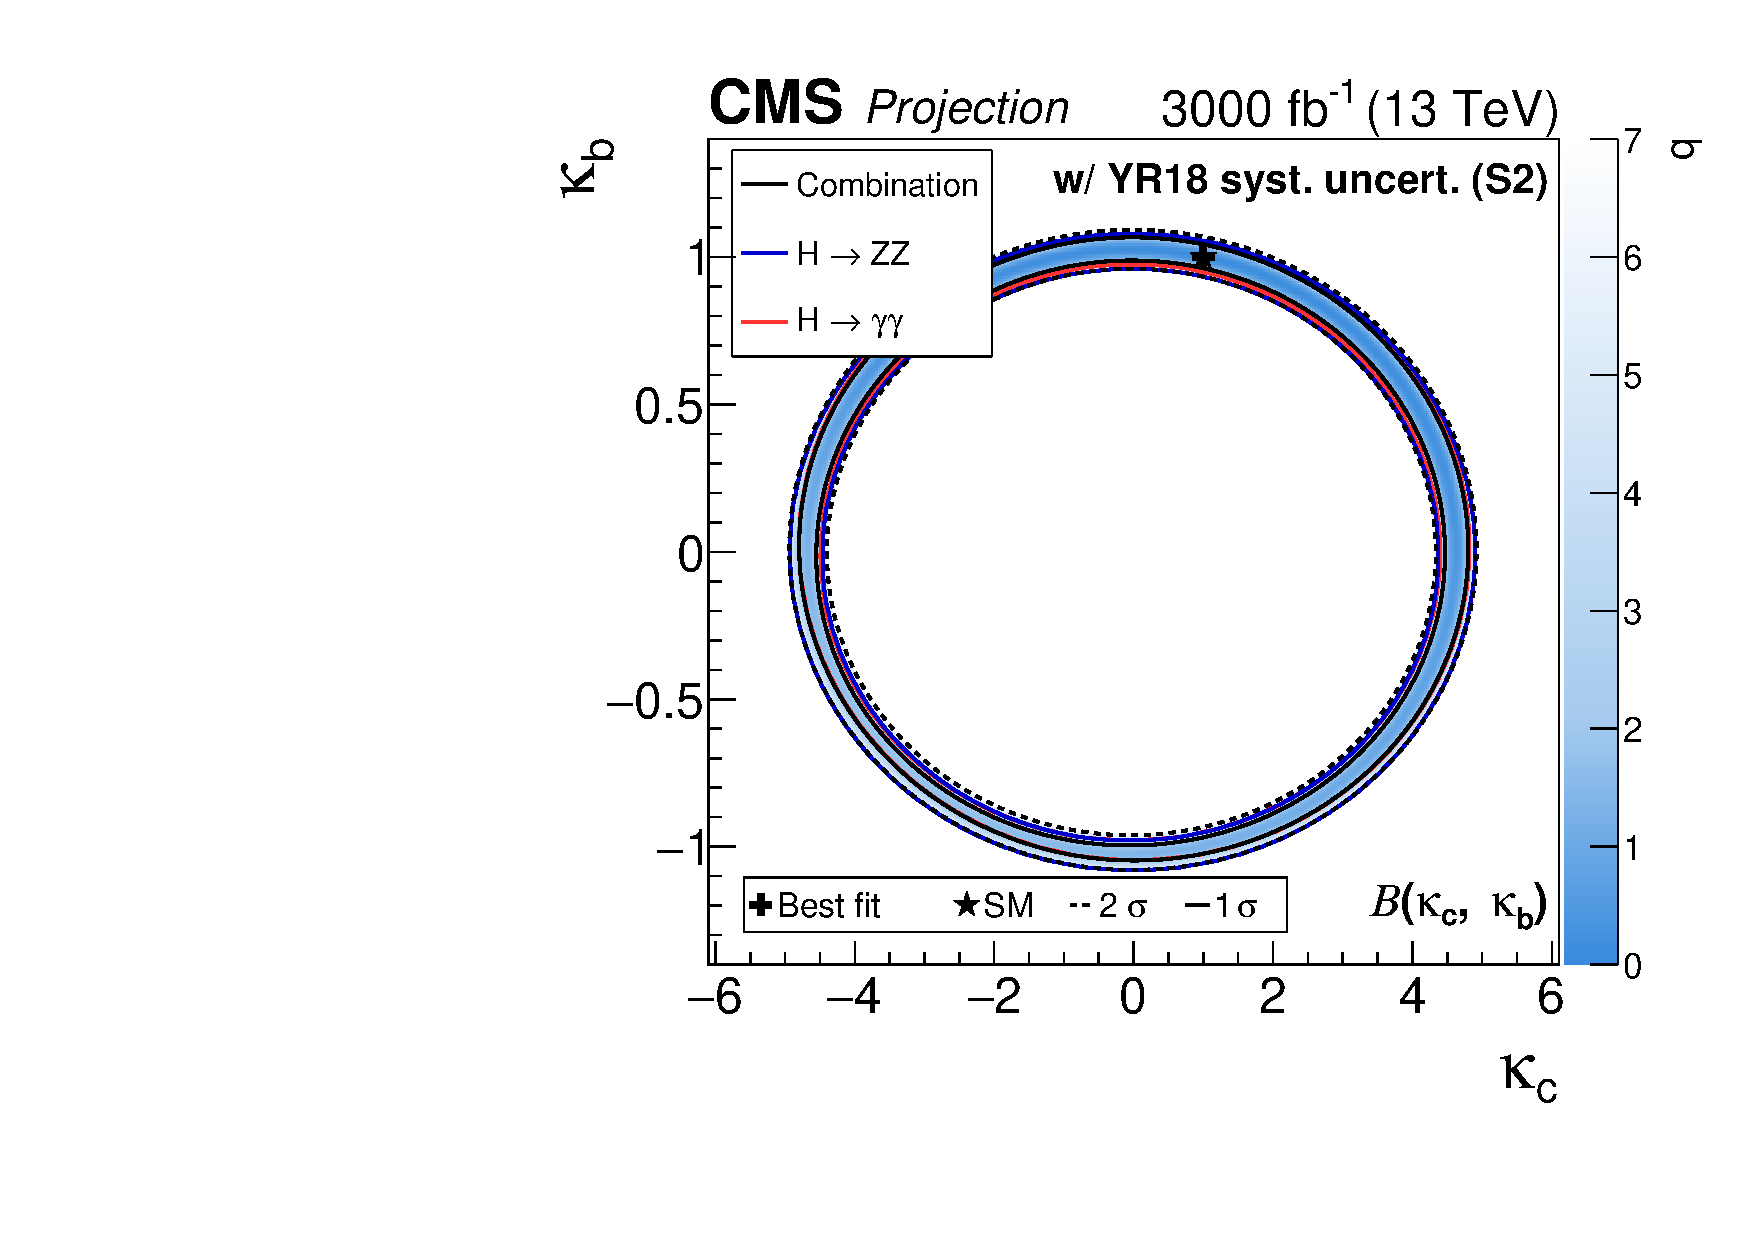
\includegraphics[width=0.49\linewidth]{img/projections/projection_kbkc_plot_couplingdependentBRs_scenario2.pdf}
        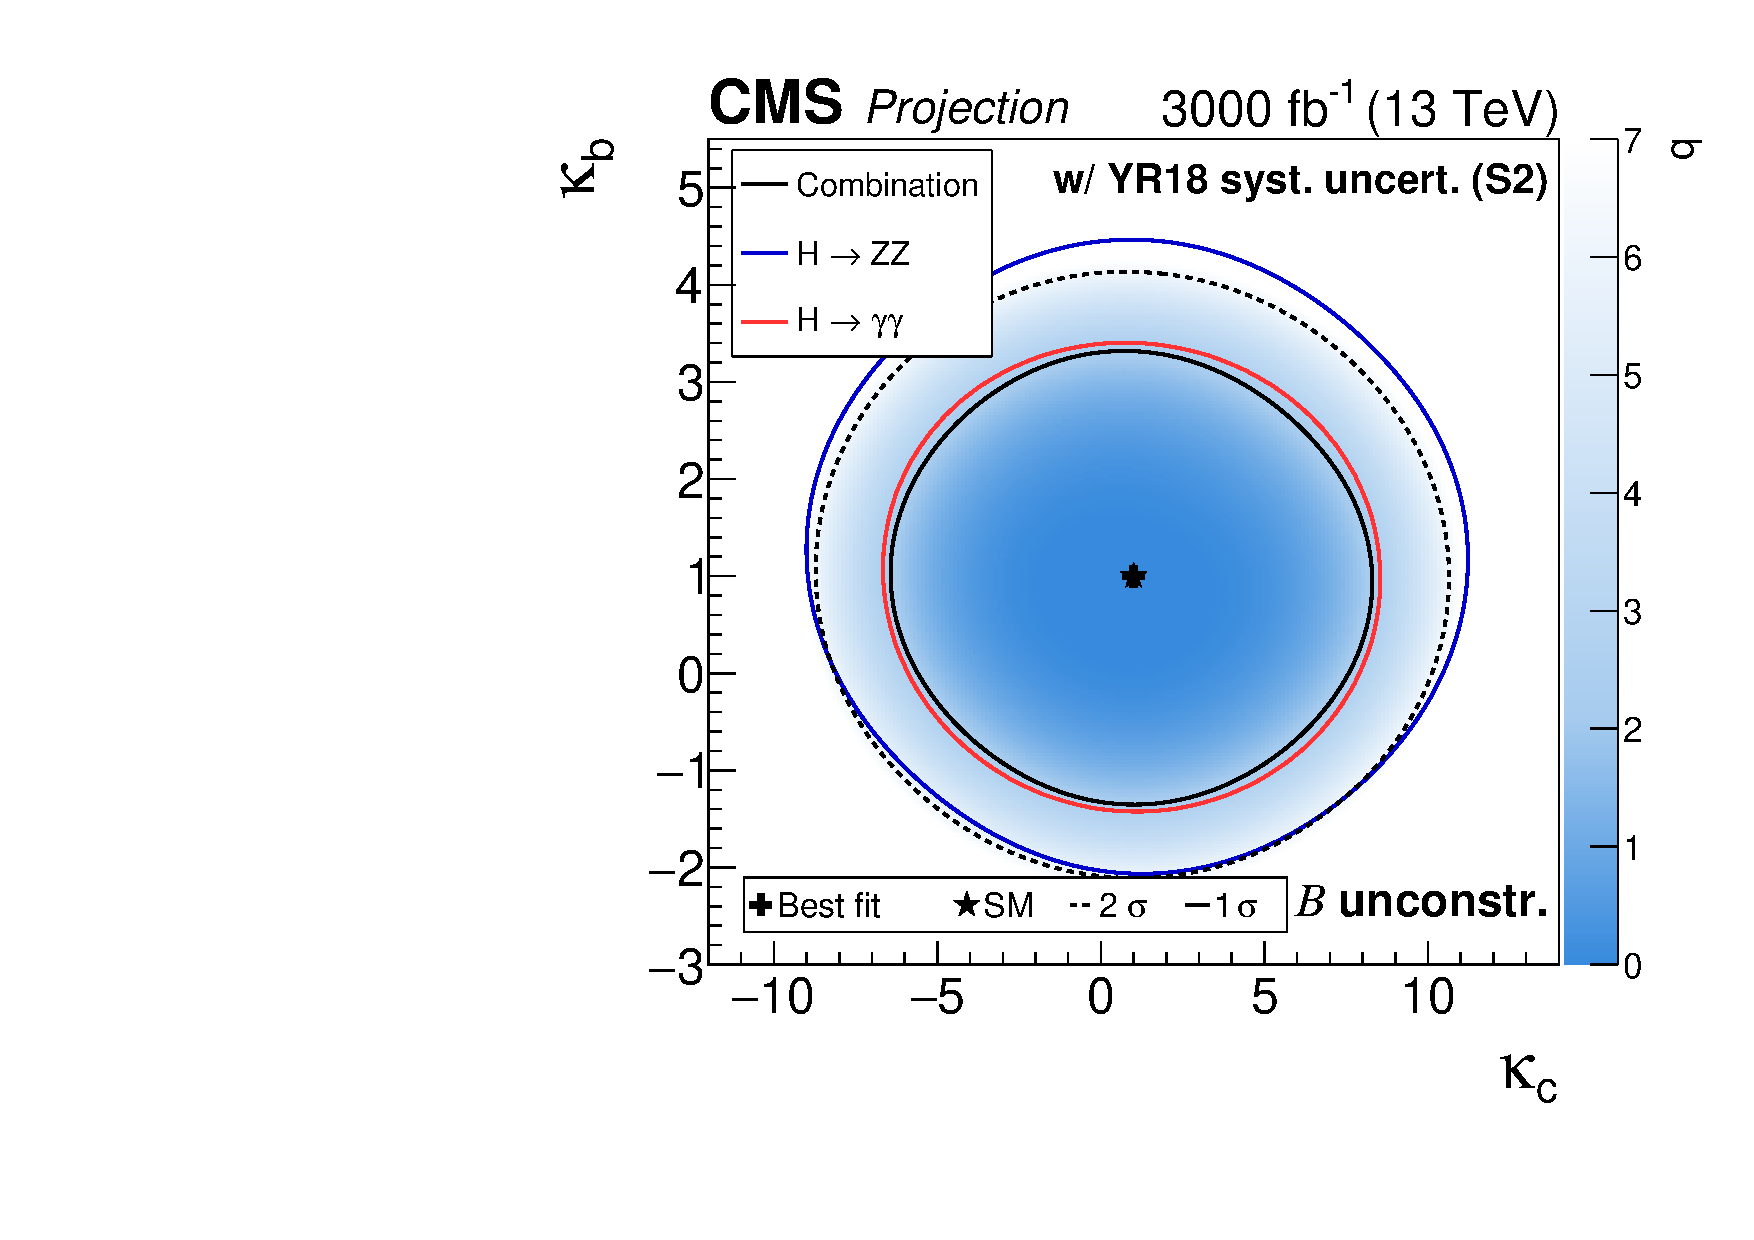
\includegraphics[width=0.49\linewidth]{img/projections/projection_kbkc_plot_floatingBRs_scenario2.pdf}
        }
    % 
    \caption{
        Projected simultaneous fit for $\kappa_\textrm{b}$ and $\kappa_\textrm{c}$, assuming a coupling dependence of the branching fractions (left) and the branching fractions implemented as nuisance parameters with no prior constraint (right), under S1 (top) and S2 (bottom).
        % 
        The one standard deviation contour is drawn for the combination ($\hgg$ and $\hzz$), the $\hgg$ channel, and the $\hzz$ channel in black, red, and blue, respectively.
        % 
        For the combination the two standard deviation contour is drawn as a black dashed line, and the shading indicates the negative log-likelihood, with the scale shown on the right hand side of the plots.
        }
    \label{fig:proj_kbkc}
  \end{center}
\end{figure}


\begin{figure}[hbtp]
  \begin{center}
    \ifbool{draftmode}{
        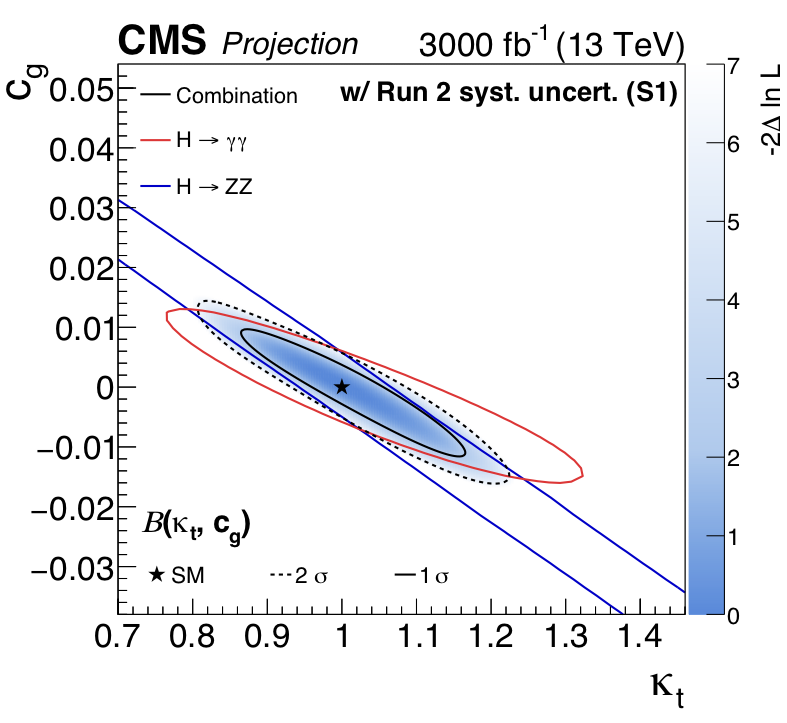
\includegraphics[width=0.49\linewidth]{img/projections/projection_ktcg_plot_couplingdependentBRs.png}
        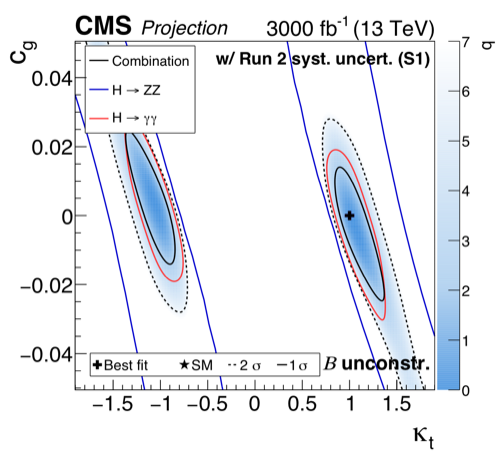
\includegraphics[width=0.49\linewidth]{img/projections/projection_ktcg_plot_floatingBRs.png}
        % 
        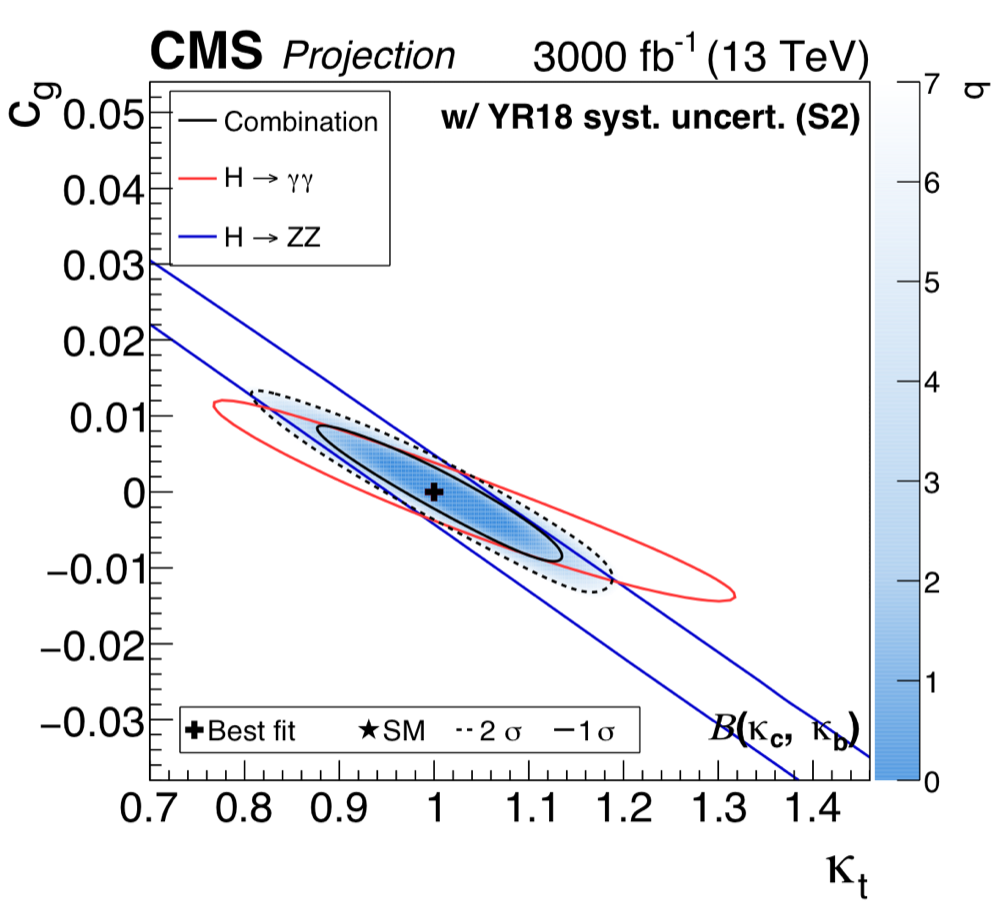
\includegraphics[width=0.49\linewidth]{img/projections/projection_ktcg_plot_couplingdependentBRs_scenario2.png}
        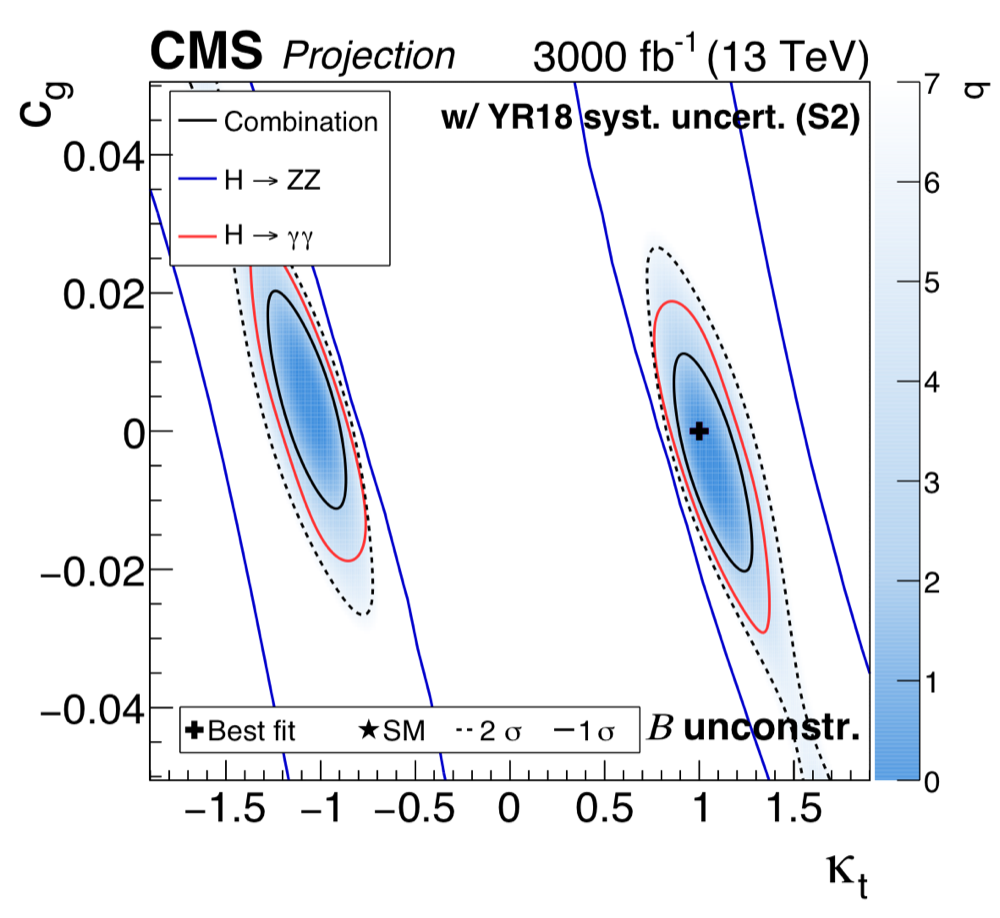
\includegraphics[width=0.49\linewidth]{img/projections/projection_ktcg_plot_floatingBRs_scenario2.png}
        }{
        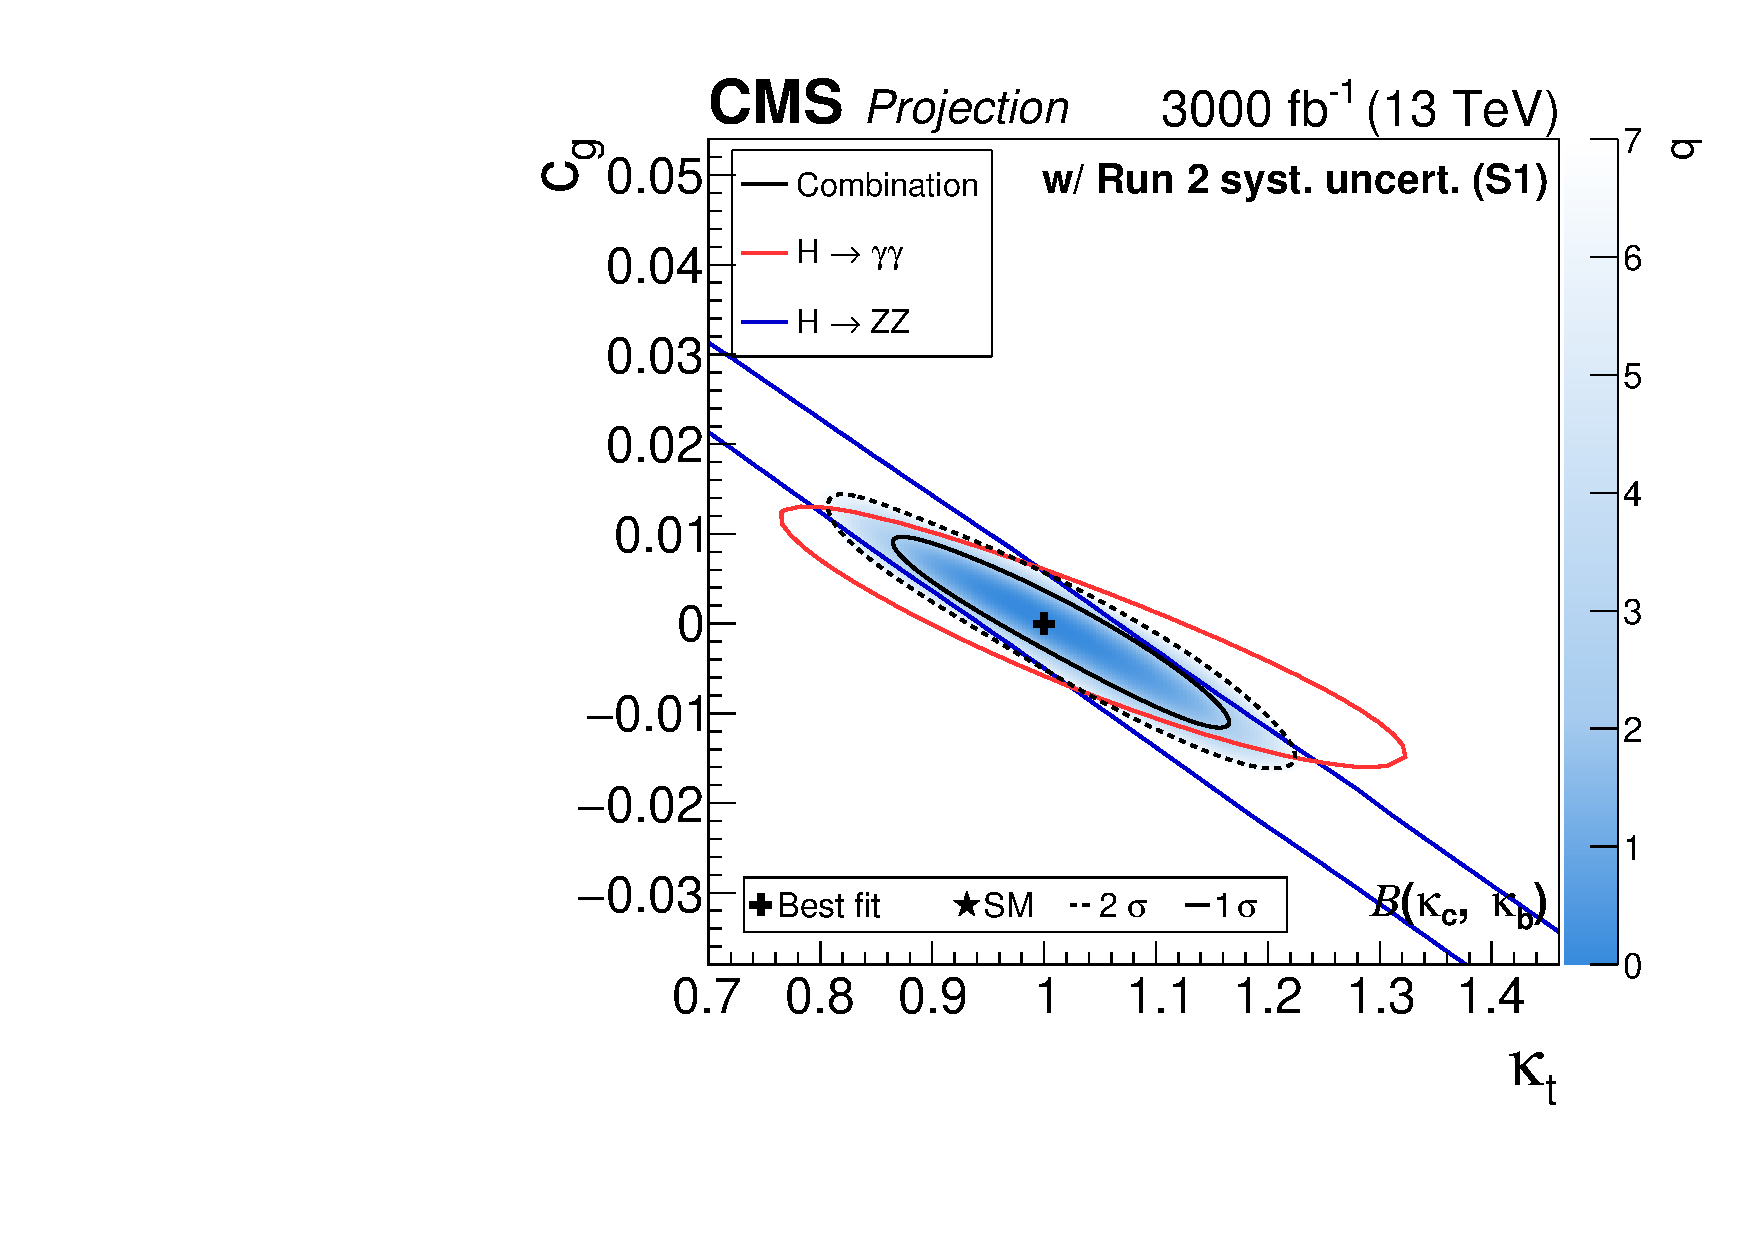
\includegraphics[width=0.49\linewidth]{img/projections/projection_ktcg_plot_couplingdependentBRs.pdf}
        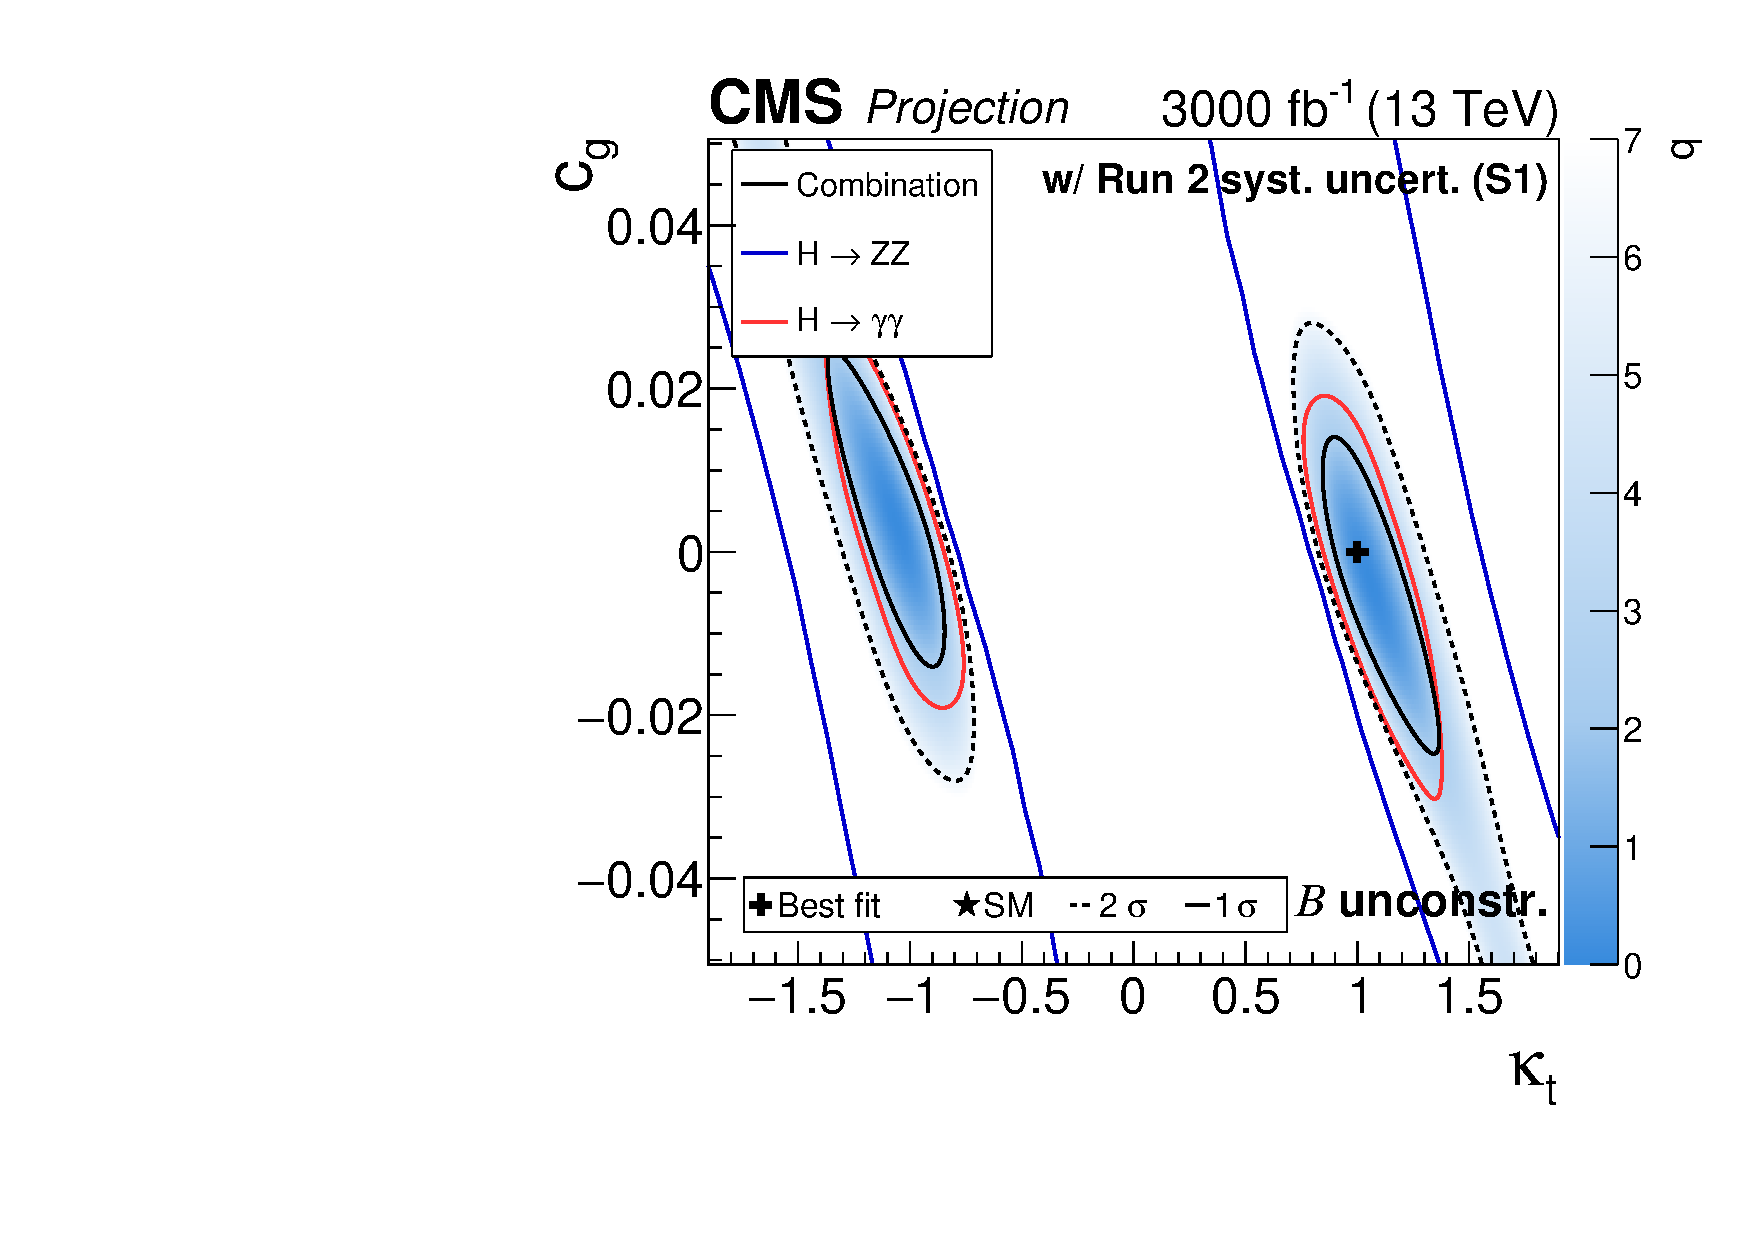
\includegraphics[width=0.49\linewidth]{img/projections/projection_ktcg_plot_floatingBRs.pdf}
        % 
        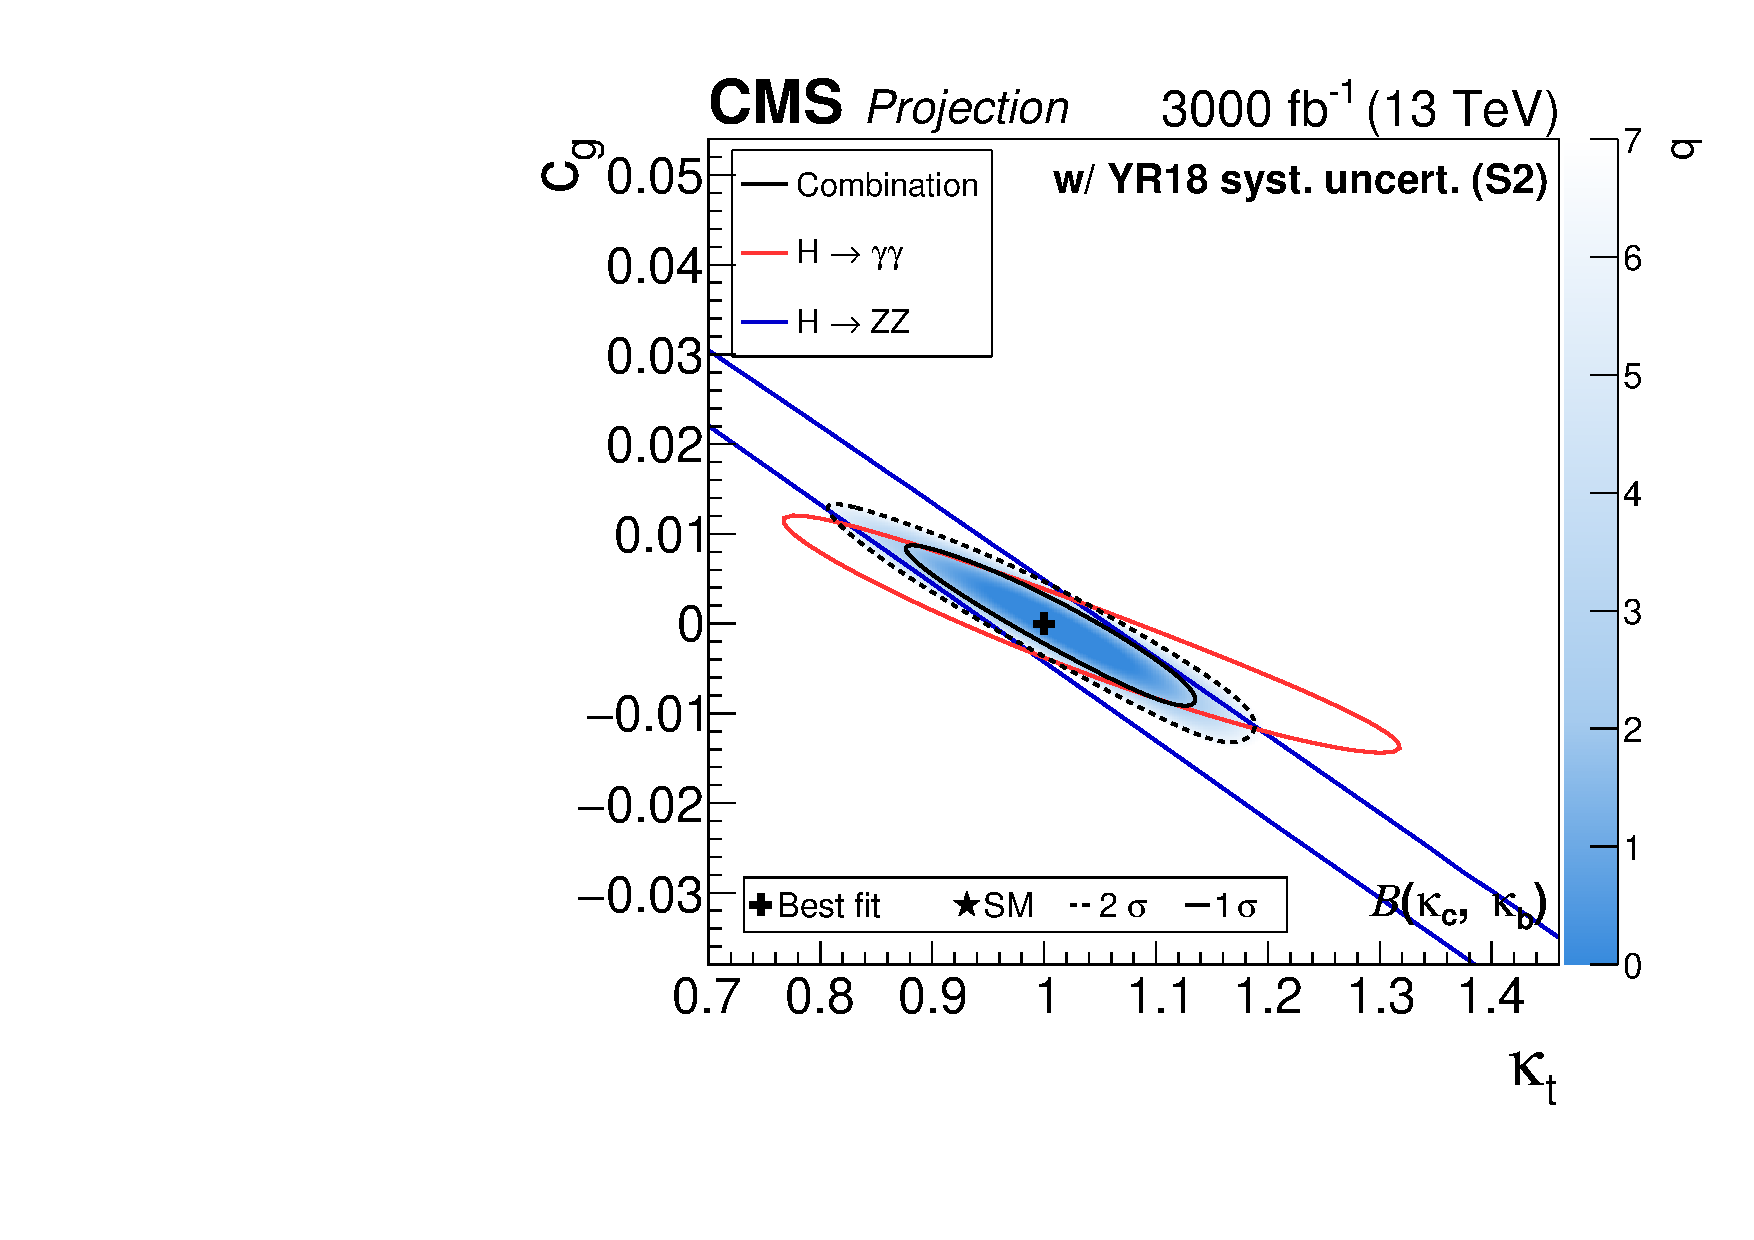
\includegraphics[width=0.49\linewidth]{img/projections/projection_ktcg_plot_couplingdependentBRs_scenario2.pdf}
        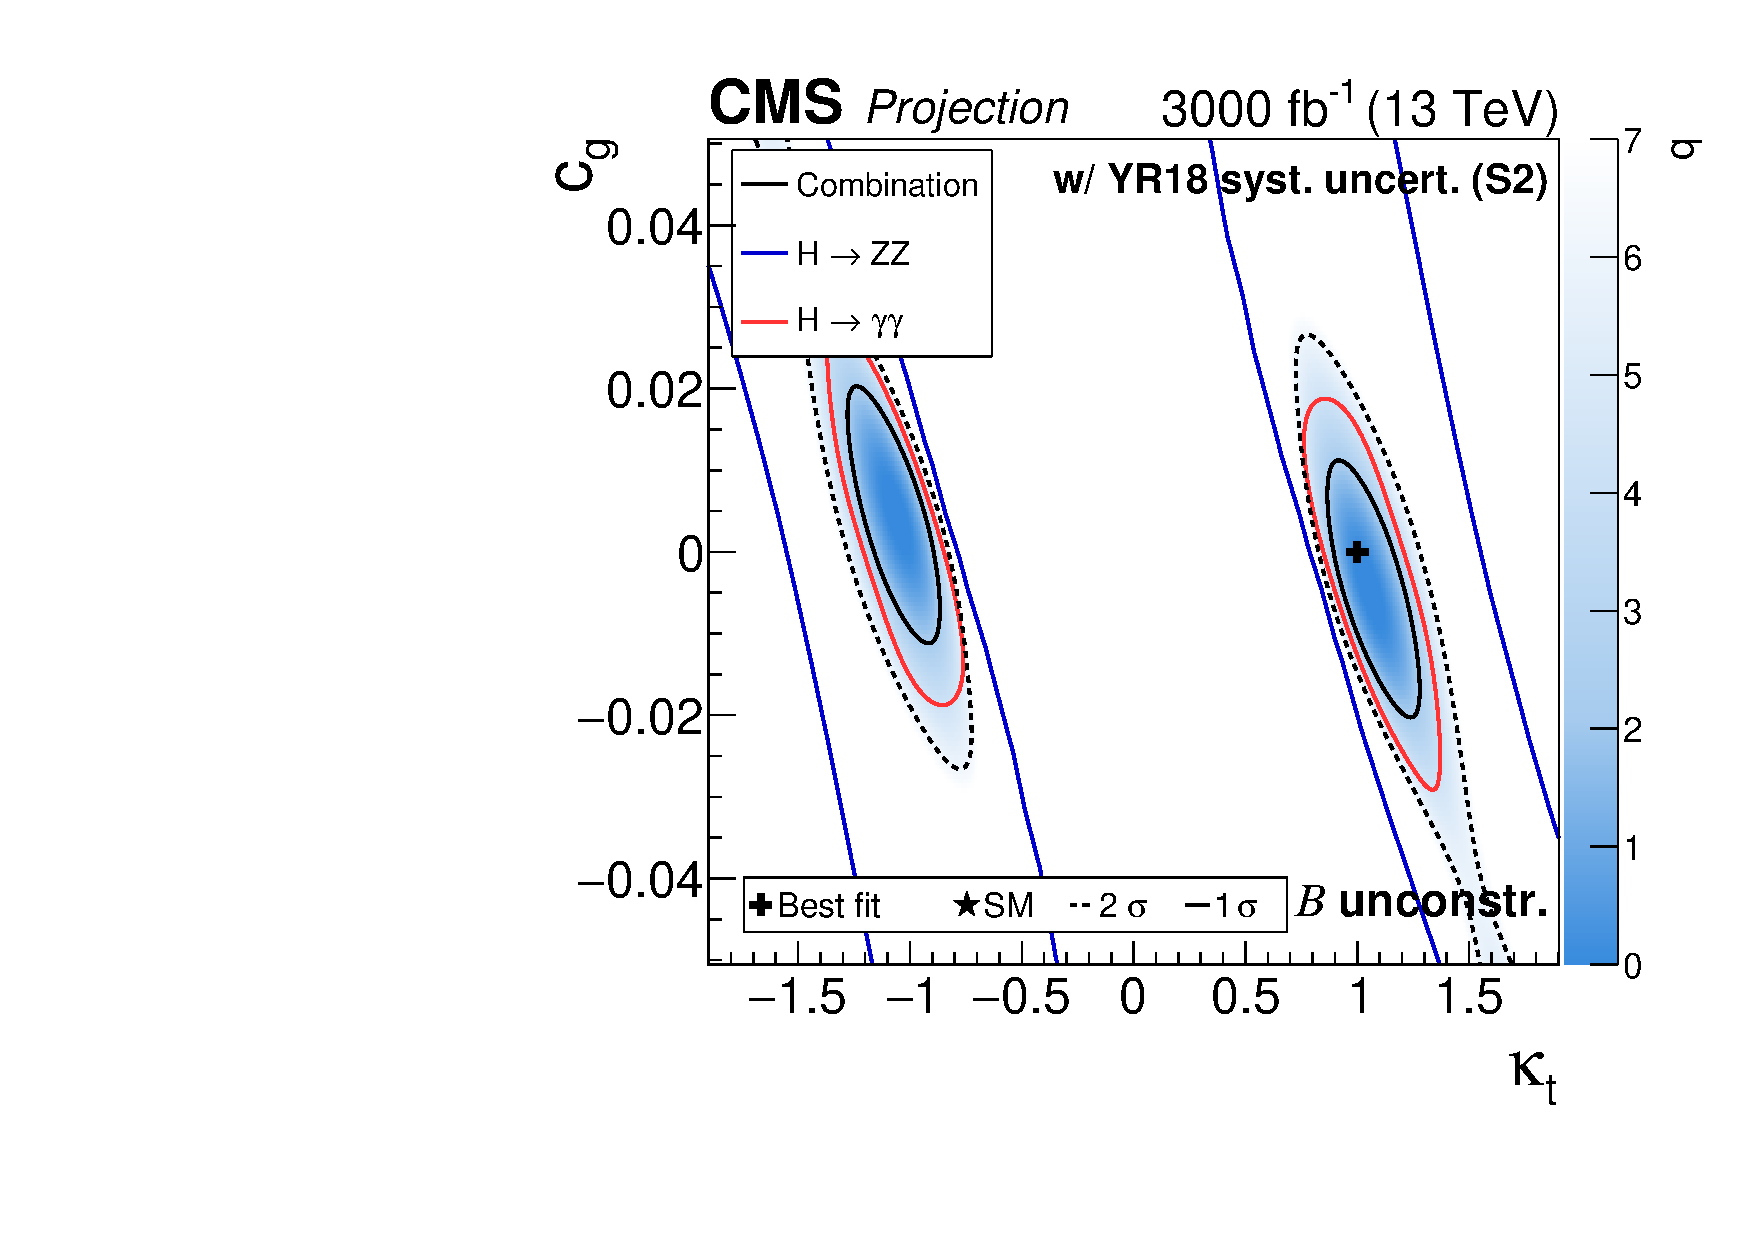
\includegraphics[width=0.49\linewidth]{img/projections/projection_ktcg_plot_floatingBRs_scenario2.pdf}
        }
    % 
    \caption{
        Projected simultaneous fit for $\kappa_\textrm{t}$ and $c_\textrm{g}$, assuming a coupling dependence of the branching fractions (left) and the branching fractions implemented as nuisance parameters with no prior constraint (right), under S1 (top) and S2 (bottom).
        % 
        The one standard deviation contour is drawn for the combination ($\hgg$, $\hzz$, and $\hbb$), the $\hgg$ channel, and the $\hzz$ channel in black, red, and blue, respectively.
        % 
        For the combination the two standard deviation contour is drawn as a black dashed line, and the shading indicates the negative log-likelihood, with the scale shown on the right hand side of the plots.
        }
    \label{fig:proj_ktcg}
  \end{center}
\end{figure}

